% !TeX spellcheck = it_IT
\documentclass[10pt,a4paper]{article}

\usepackage[utf8]{inputenc}
\usepackage[T1]{fontenc}	
\usepackage[italian]{babel}
\usepackage{amsmath}
\usepackage{amsfonts}
\usepackage{amssymb}
\usepackage{graphicx}

\usepackage[left=2cm,right=2cm,top=2cm,bottom=2cm]{geometry}
\geometry{a4paper}

\usepackage{booktabs} % for much better looking tables
\usepackage{verbatim}
\usepackage{subfig} % make it possible to include more than one captioned figure/table in a single 

\usepackage{fancyhdr} % This should be set AFTER setting up the page geometry
\pagestyle{fancy} % options: empty , plain , fancy
\renewcommand{\headrulewidth}{0pt} % customise the layout...
\lhead{}\chead{}\rhead{}
\lfoot{}\cfoot{\thepage}\rfoot{}

%%% SECTION TITLE APPEARANCE
\usepackage{sectsty}
%\allsectionsfont{\sffamily\mdseries\upshape} % (See the fntguide.pdf for font help)
% (This matches ConTeXt defaults)

% pacchetti che mi fanno schifo ma uso lo stesso (Bob è scemo...)
\renewcommand{\square}{ciao}
\usepackage[cdot, thickqspace, squaren]{SIunits}
% macro che mi piacciono
\def\code#1{\texttt{#1}}


\title{Esercitazione 5: Transistor JFET}

\author{Gruppo BE \\ Alessandro Candido, Roberto Ribatti}
\date{\today}
\begin{document}
\maketitle

\section{Scopo e strumentazione}
Studiare le caratteristiche e realizzare un amplificatore con il JFET a canale N 2N3819.
La strumentazione usata è quella presente sul banco di lavoro, più il suddetto transistor.

\section{Studio del funzionamento del JFET}

\subsection{Dimensionamento}
Si è montato il circuito in \figurename{\ref{fig:circuito1}}.

\begin{figure}[h!]
	\centering
	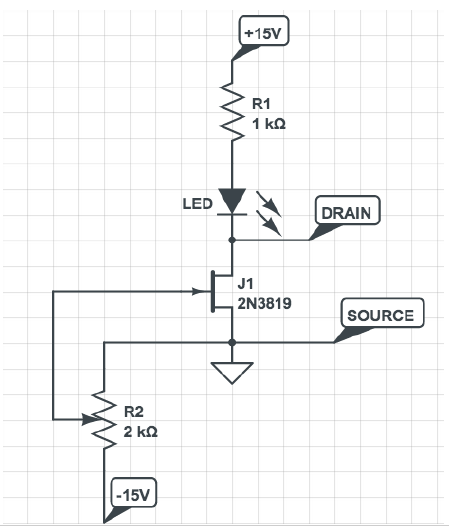
\includegraphics[width=0.5\textwidth]{../grafici/Circuito1.png}
	\caption{Circuito per lo studio del funzionamento del JFET}
	\label{fig:circuito1}
\end{figure}

I valori dei componenti usati sono stati misurati con il multimetro.

\begin{table}[h!]
	\centering
	\begin{tabular}{ccc}
		$V_{15} = \unit{15.0 \pm 0.2}{\volt}$  & $V_{-15} = \unit{-15.0 \pm 0.2}{\volt}$ & $R_1 = \unit{985 \pm 9}{\ohm}$
	\end{tabular}
\end{table}

\paragraph{LED} Il LED si accende e si spegne alla tensione $V_{GS} \sim \unit{1.89}{\volt}$. Infatti al di sopra di una certa tensione gate-source ($V_{GS}$) il canale è da considerarsi chiuso (pinch-off) e il transistor va in interdizione. Al di sotto della tensione di pinch-off a corrente inizia a scorrere nel canale, portando in conduzione anche il LED.

\subsection{Tensione di pinch-off $V_P$ e massima corrente di drain $I_{DSS}$}
I dati relativi alla curva $I_D - V_{GS}$ sono riportati in appendice in \tablename{\ref{njfet}}, il grafico relativo è invece riportato di seguito (\ref{fig:njfet}).

Si è trovato per la tensione di pinch-off il valore di $ $, mentre per la massima corrente di drain $ $.
% il valore sarà quello relativo alla corrente di 0.5uA; va notato che non c'è solo un errore sulla misura relativa alla tensione, ma c'è anche un errore dovuto a quanto è 0 la corrente di 0.5uA (entro l'errore lo è, ma magari con una misura più precisa quella corrente non sarebbe stata nulla e quindi anche la tensione sarebbe diversa, mantenendo il suo errore), andrebbe propagato anche quest'errore.
%stessa cosa per idss
%queste considerazioni espresse meglio andrebbero poi scritte nella relazione

%includere il grafico

\section{Montaggio amplificatore}

\subsection{Dimensionamento}

I valori dei componenti usati nel circuito in \figurename{\ref{fig:amplificatore}} sono:

\begin{table}[h!]
\centering
\begin{tabular}{cccc}
$R_1 = \unit{985 \pm 9}{\ohm}$ & $R_3 = \unit{4.65 \pm 0.07}{\mega\ohm}$ & $R_{trim} = \unit{244 \pm 3}{\ohm}$ & $ C_1 = \unit{101 \pm 5}{\nano\farad}$
\end{tabular}
\end{table}

Si è indicato con $R_{trim}$ la resistenza del trimmer al punto di lavoro fissato (si veda paragrafo seguente).

\begin{figure}[h!]
	\centering
	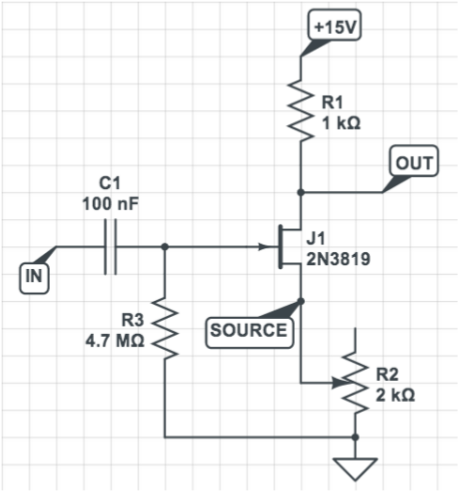
\includegraphics[width=0.5\textwidth]{../grafici/amplificatore.png}
	\caption{Schema del circuito dell'amplificatore a JFET (common source o source follower)}
	\label{fig:amplificatore}
\end{figure}

\paragraph{Punto di lavoro} Si è montato l'amplificatore, rappresentato in \figurename{\ref{fig:amplificatore}}, imponendo il punto di lavoro in modo tale che la corrente di drain $I_D$ fosse $\sim I_{DSS}/2$. Il valore misurato è $I_D = \unit{3.05 \pm 0.03}{\milli\ampere}$.

%I valori misurati per tensione drain-source e corrente di drain sono riportati di seguito.
%\begin{table}[h!]
%\centering
%\begin{tabular}{cc}
%$V_{DS} = \unit{650 \pm 4}{\volt}$ & $I_{DS} = \unit{3.05 \pm 0.03}{\milli\ampere}$
%\end{tabular}
%\end{table}

\paragraph{Verifica del punto di lavoro} Si è misurato inoltre $V_{GS} = \unit{650 \pm 4}{\volt}$ e si è calcolato il valore atteso per la corrente di drain $I_D$ secondo la formula:
\begin{equation*}
I_D = \frac{I_{DSS}}{V_P^2}(V_{GS} - V_P)^2
\end{equation*}

Ottenendo quindi $I_D^{exp} = \unit{3.07 \pm 0.04}{\milli\ampere}$. Si ottiene inoltre per la transconduttanza il valore di $g_m = \unit{4.00 \pm 0.05}{\milli\Siemens}$
%i valori sono ottenuti con Vp e Idss presi a spanne con errori dal multimetro, poi lo aggiorno, comunque sono già compatibili

\section{Misure a frequenza fissa}

Si è misurato il guadagno in risposta a segnali sinusoidali di frequenza fissa pari a $\unit{1.011 \pm 0.010}{k\hertz}$ nella configurazione di common source e source follower

\paragraph{Fase relativa tra ingresso e uscita} Si è osservato che il segnale in uscita risultava in opposizione di fase rispetto al segnale in ingresso nel caso della configurazione common source e in fase nel caso della configurazione follower source, come atteso. Si riporta in \figurename{\ref{fig:controfase}} e \figurename{\ref{infase}} le relative schermate dell'oscilloscopio.

\begin{figure}[h!]
	\centering
	\begin{minipage}[h!]{0.5\textwidth}
		\centering
		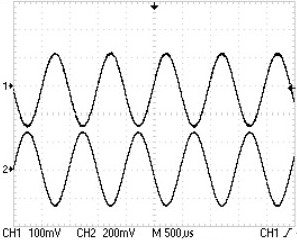
\includegraphics[width=\textwidth]{../oscilloscopio/inversione_fase.jpg}
		\caption{common source}
			\label{fig:controfase}
	\end{minipage}
	\begin{minipage}[h!]{0.49\textwidth}
		\centering
		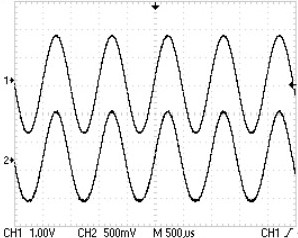
\includegraphics[width=\textwidth]{../oscilloscopio/fase.jpg}
		\caption{source follower}
			\label{infase}
	\end{minipage}

\end{figure}

\paragraph{Guadagno e linearità del circuito} Si è fittato il guadagno in tensione del circuito $|A_V|$ ottenendo i seguenti risultati:
\begin{table}[h!]
	\centering
	\begin{tabular}{cccc}
		common source & $|A_v| = 1.996 \pm 0.019$ & intercetta: $\unit{0.005 \pm 0.008}{\volt}$ & $\chi^2 / ndof = 25.5 / 22$\\
		source follower &	$|A_v| = 0.467 \pm 0.004$ & intercetta: $\unit{0.0025 \pm 0.0012}{\volt}$ & $\chi^2 / ndof = 21.3 / 23$
	\end{tabular}
\end{table}

Il valore atteso dalla teoria è di

\begin{table}[h!]
	\centering
	\begin{tabular}{cc}
		common source & $|A_v| =g_mR_D/(1+g_mR_S) =$ \\
		source follower &	$|A_v| =g_mR_S/(1+g_mR_S) = $
	\end{tabular}
\end{table}

Sono entrambi compatibili con quelli misurati entro $\sigma$.
I grafici dei fit sono riportati di seguito, mentre i dati raccolti sono in appendice in \tablename{\ref{commonsource}} e \tablename{\ref{sourcefollower}}

\begin{figure}[h!]
	\centering
	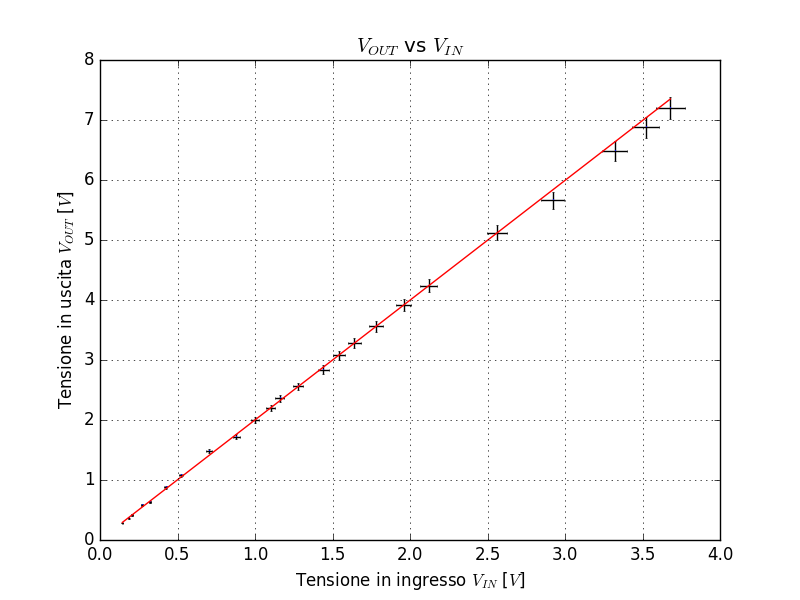
\includegraphics[width=0.8\textwidth]{../grafici/fit_guadagnovstensione.pdf}
	\caption{Grafico del fit del guadagno del circuito common source}
\end{figure}
\begin{figure}[h!]
	\centering
	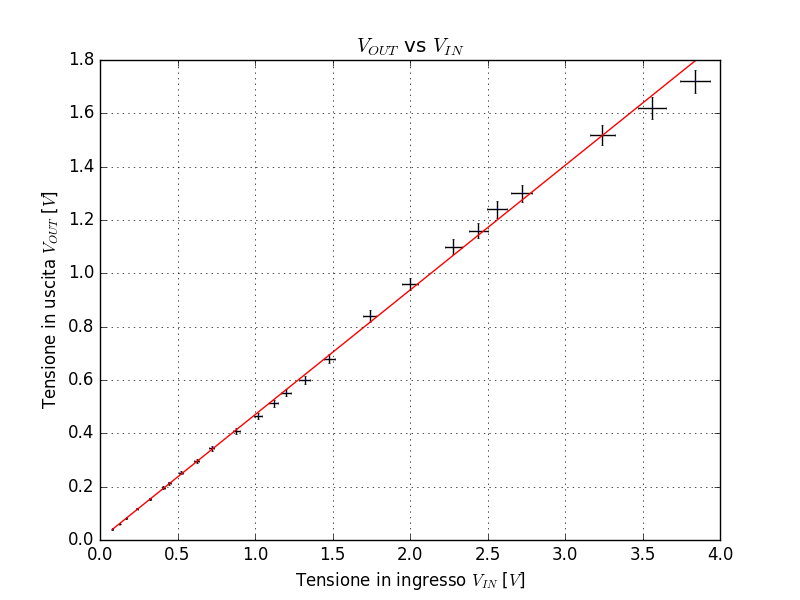
\includegraphics[width=0.8\textwidth]{../grafici/fit_guadagnovstensione2.pdf}
	\caption{Grafico del fit del guadagno del circuito source follower}
\end{figure}

 Si può affermare che la linearità è preservata per le tensioni d'ingresso che non portano il transistor in clipping.
  
 \paragraph{Clipping}
Il segnale in uscita risulta sinusoidale fino ad ampiezze di $\sim \unit{4.4}{\volt}$ in ingresso per entrambe le configurazioni.
Per intensità maggiori si osserva che l'uscita è tagliata dall'alto nel common source e dal basso nel source follower. Questo taglio del segnale (riportato in \figurename{\ref{fig:clippingalto}} e \figurename{\ref{fig:clippingbasso}}) corrisponde ad un regime di funzionamento del transistor diverso da quello attivo, in cui sarebbe preservata la linearità.

\begin{figure}[h!]
	\centering
	\begin{minipage}{0.49\textwidth}
		\centering
		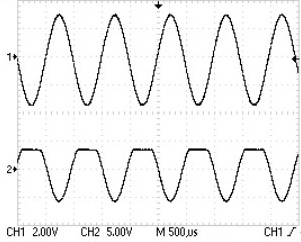
\includegraphics[width=\textwidth]{../oscilloscopio/clipalto.jpg}
		\caption{Clipping common source}
			\label{fig:clippingalto}
	\end{minipage}
	\begin{minipage}{0.49\textwidth}
		\centering
		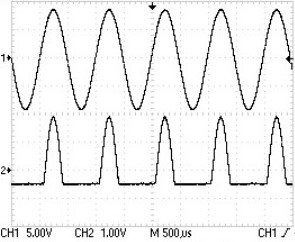
\includegraphics[width=\textwidth]{../oscilloscopio/clipping basso.jpg}
		\caption{Clipping source follower}	
			\label{fig:clippingbasso}	
	\end{minipage}
\end{figure}

\section{Impedenza d'ingresso}

\section{Aumento del guadagno}

\pagebreak
\section{Appendice: Dati}
Si riportano qui le tabelle di dati usati per i fit e i grafici.

\begin{figure}[h]
	\centering
	\begin{minipage}[c]{0.4\textwidth}
		\centering
		%\input{../tabelle/tab_guadagnopiccolisegnali_ol.txt}
		\captionof{table}{Curva $I_D - V_{GS}$}
		\label{njfet}
	\end{minipage}
	\begin{minipage}[c]{0.4\textwidth}
		\centering
		%\input{../tabelle/tab_f_domain.txt}
		\captionof{table}{}
		\label{}
	\end{minipage}
\end{figure}

\end{document}
